\chapter{序論}

\section{重陽子-陽子弾性散乱を用いた3体核力の研究}
\section{重陽子-陽子弾性散乱に向けた偏極陽子標的の開発}
偏極重陽子-陽子弾性散乱によるスピン観測量の高精度測定のために、偏極固体陽子標的として低磁場($\sim 0.3$ T)下で項偏極度($\sim 30\%$)を達成することが求められる。
我々はこれらの条件を達成可能な偏極陽子標的の開発を行ってきた。
まず、偏極手法として光励起三重項電子スピンを用いた動的核偏極(Triplet-DNP)を採用した。
Triplet-DNPは低磁場($\sim 0.3$ T)高温(>100 K)環境で固体陽子標的の偏極を行うことができる手法である。
また、標的試料として重水素化ペンタセン($C_{22}D_{14}$)をドープしたナフタレン($C_{10}H_8$)単結晶を採用した。
図にナフタレンと重水素化ペンタセンの構造式を示す。ナフタレンは散乱実験の偏極陽子標的として使用された実績があり、Triplet-DNPを偏極手法として100 K,0.3 Tの環境下で約$37\%$の偏極度を達成したことが報告されている。\\

\section{陽子-陽子弾性散乱における放射損傷による減偏極の観測}
2022年量研HIMACで200 MeV陽子ビームを用いた陽子-陽子弾性散乱実験を実施し、その際ナフタレン標的において減偏極が観測された。
要因として、ビームと標的結晶との相互作用により結晶構造が破壊されることでスピン-格子緩和時間$T_1$が短くなり、
到達偏極度が低くなることが挙げられる。
また、ビーム照射によって標的結晶の温度が上昇し、$T_1$が短くなっていることも減偏極の要因として考えられる。
本論では、結晶構造の破壊によって蓄積される緩和要因を「積分効果」、温度上昇によってビーム照射中にのみ存在する緩和要因を「強度効果」と呼称し、減偏極のデータをもとに各要因の評価を行う。
% 核力は核子同士を結びつけ原子核を構成する基本的な力である。この核力を理論的に理解し、原子核という有限量子多体系を理解することは、原子核物理学における重要な課題の一つである。この章では現在までに行われてきた核力研究の経緯や、それによって明らかになってきた三体核力の重要性およびその実験的検証について述べる。また我々の研究グループがこれまで行ってきた研究状況および本研究の目的についても述べる。

% %%%% 1.1 %%%%
%  \section{核力の研究}
% %% 1.1.1 %%
%   \subsection{核力}
% 到達距離がほぼ無限大である重力や電磁気力と異なり、核力の到達距離は$10^{-15}$ m($1~{\rm fm}$)のオーダーと極端に短い。この到達距離の範囲内では電磁気力の$100$倍程度の強い力がはたらき、陽子や中性子を$10^{-14}$ m程度の非常に狭い空間に束縛している。この核力の理論的記述は、有限の質量を持った粒子を媒体とする量子化された場を導入するという形で、1935年に湯川秀樹によって初めて与えられた\cite{yukawa}。また湯川は、$2~{\rm fm}$程度の核力の到達距離を表すために、この粒子は核子と電子の中間の質量($\sim 100~{\rm MeV}$)を持つと予言した。このことから、この粒子は“中間子”と呼ばれるようになった。後にこの中間子($\pi$中間子、パイオン)はOcchialiniらによって、宇宙線観測から存在が確認された\cite{Occ47}。\\
%  二つの核子間の距離が$2~{\rm fm}$以上の比較的遠距離の領域では、1個の$\pi$中間子の交換(one-pion exchange, OPE)による相互作用が支配的となる。$2~{\rm fm}$以下の領域になると、複数個の$\pi$中間子交換や、より質量の大きい他の中間子($\rho$中間子、$\omega$中間子等)の交換による相互作用等の寄与が生じる。1960年代になると、この重い中間子による寄与を考慮した1ボソン交換(one-boson exchange, OBE)模型が発展した。この模型は湯川の理論に基づき、様々な中間子1個の交換の寄与を足し合わせることで核力を記述するものである。また同年代において、実験側では世界中の加速器施設で核子--核子弾性散乱実験が行われた。60年代の終わりにはこれらの実験で得られた$450~{\rm MeV}$までのおよそ2000個の核子--核子散乱データについての位相シフト解析が行われた\cite{MAW69}。70年代から80年代にかけては、核子共鳴も含んだ複数のパイオンの交換模型が発展し、87年には包括的な中間子交換模型(Bonn full model \cite{MHE87})が完成した。

% %%%%%%%

% %% 1.1.2 %%
%   \subsection{現実的な核力ポテンシャル}
% 実験や理論研究の更なる進展により、90年代には幾つもの現実的な核力ポテンシャルが完成した。代表的なものとしては、Argonne $v_{18}$ポテンシャル(AV18 \cite{WJS95})、CD-Bonnポテンシャル(CD-Bonn \cite{Mac01})、Nijmegenポテンシャル(Nijmegen I,II \cite{Sto94})が挙げられる。これらの核力ポテンシャルは 90年代までに蓄積された計5000個以上の高精度かつ膨大な核子-核子散乱実験データを$\chi^2/N_{\rm data} \sim 1$という精度で再現している。このことから、二つの核子間で働く二体核力に関してはほぼ確立したといえる。

% %%%%%%%

% %%%% 1.2 %%%%
%  \section{三体核力の研究}
% %% 1.2.1 %%
%   \subsection{三体核力}
% 実際の原子核は多数の核子によって構成されているため、複数個の核子間で作用する多体力の効果は核力を記述する上で必要不可欠なものと考えられてきた。三体核力の存在自体は1933年に Wignerによって初めて示唆された\cite{Wig33}。1961年にはFaddeevによって量子力学的に三体問題を厳密に記述する理論が提唱され\cite{Fad61}、以後この理論に基づいた三核子系の束縛エネルギーを記述する試みが行われるようになった。二体核力ポテンシャルのみを用いた三重水素(${}^3$H)の束縛エネルギーの計算では実験値より$1~{\rm MeV}$程度小さくなることから、三体核力の効果を考慮することでこの不一致が解消されるものと期待された\cite{IS86,Che86}。近年では、${}^3$Hや${}^3$Heなどの三核子系だけでなく$\alpha$粒子などの四核子系の束縛エネルギーも三体核力の効果によって実験値を再現することが示されている\cite{Nog02}。\\
%  最初の三体核力の理論モデルは、1957年に藤田と宮沢によって与えられた$2\pi$交換型の三体核力モデルである\cite{FM57}。図\ref{FMmodel_FD}にこの藤田-宮沢型三体核力モデルのFeynman図を示す。図のように、 3つの核子間で2つの$\pi$中間子を核子の$\Delta$励起を介して交換している。このような反応は二体核力のみでは記述することができず、3つの核子があって初めて考えられる反応である。

% \begin{figure}[tbp]
%  \centering
%  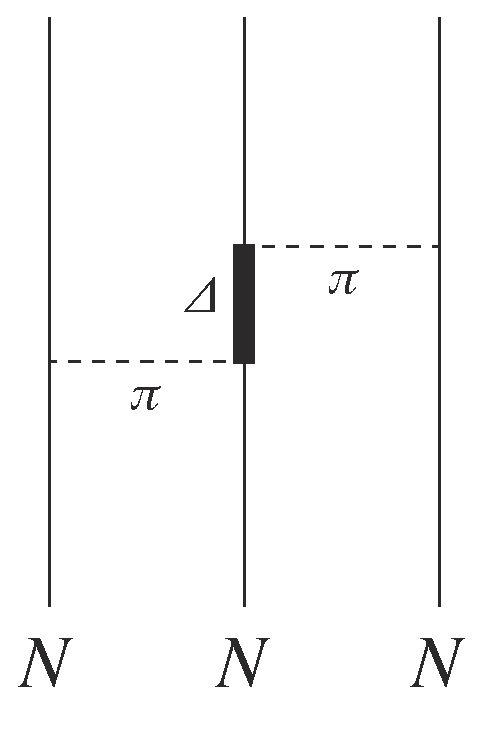
\includegraphics[clip,width=4cm]{./chap1/fig/3NF_2pi-model.pdf}\\
%  \caption{藤田-宮沢型三体核力モデルのFeynman図}
%  \label{FMmodel_FD}
% \end{figure}

% 現在用いられている主な三体核力のモデルとしてはUrbana IX\cite{Pud97}やTucson-Melbourne'99\cite{CH01}型がある。これらのモデルも藤田-宮沢型同様$2\pi$交換型の三体核力を主成分としたものである。

% %%%%%%%

% %% 1.2.2 %%
%   \subsection{散乱系における三体核力}
% 核力は運動量依存性およびスピン・アイソスピン依存性を持つ。よって、三体核力を含む核力の性質を詳細に調べる手段としては少数核子系散乱が非常に有効なプローブである。散乱実験によって三体核力の状態依存性を明確にすることは、その性質を調べていく上で重要である。\\
%  前述した二体核力の現実的な核力ポテンシャルおよび計算機の性能の向上により、近年では少数核子系の散乱における観測量について、モデルに依存しない厳密理論計算が可能となった。最も単純な三核子系散乱である核子--重陽子散乱については、低エネルギー領域において高精度の実験データとFaddeev方程式に基づく厳密理論計算との比較が行われた\cite{Glo96,KVR01}。その結果、核子当たり約30 MeV以下の低エネルギーではベクトル偏極分解能を除くほぼすべての観測量が二体核力のみを用いた計算で再現された。よって、低エネルギー領域においては三体核力の効果が二体核力に比べて非常に小さく、散乱実験によってその効果の寄与を観測することは困難であることが分かった。一方で、核子当たりの入射エネルギーがより大きくなると三体核力の効果も相対的に大きくなることが示唆された。\\
%  1998年には、Wita{\l}aらによって核子当たり約60 MeVにおける核子--重陽子散乱において三体核力の効果が現れることが理論的に初めて指摘された\cite{Wit98}。Wita{\l}aらの理論グループはTM型の三体核力モデルを含むFaddeev厳密理論計算を行い 、核子--重陽子弾性散乱における微分断面積が最小値を取る角度で三体核力の効果が顕著に現れることを示した。\\
%  理化学研究所のグループは、中間エネルギー領域での重陽子--陽子弾性散乱実験を行い、それによって得られた精緻な実験データから、理論的に予想された散乱系における三体核力の寄与大きさがほぼ正しいことを初めて明らかにした\cite{Sek02,Sek11}。例として、核子当たり135 MeVでの微分断面積の実験データおよび理論計算を図\ref{dcs_dp135}に示す。白丸が実験データ、青い帯が二体核力の核力ポテンシャル(AV18, CD-Bonn, Nijmegen I,II)のみを用いた理論計算であり、赤い帯が二体核力に三体核力(TM'99型)を入れ込んだ理論計算である。黒線は二体核力のAV18に三体核力であるUrbana IXを加えた理論計算である。理論計算による三体核力の寄与が重心系での散乱角度$\theta_{\rm c.m.} \sim 120^\circ$で現れている。この散乱角度では実験データが二体核力のみの理論計算よりも30%程度大きい値を取っているが、三体核力を考慮することで実験データを良く再現していることが分かる。

% \begin{figure}[tbp]
%  \centering
%  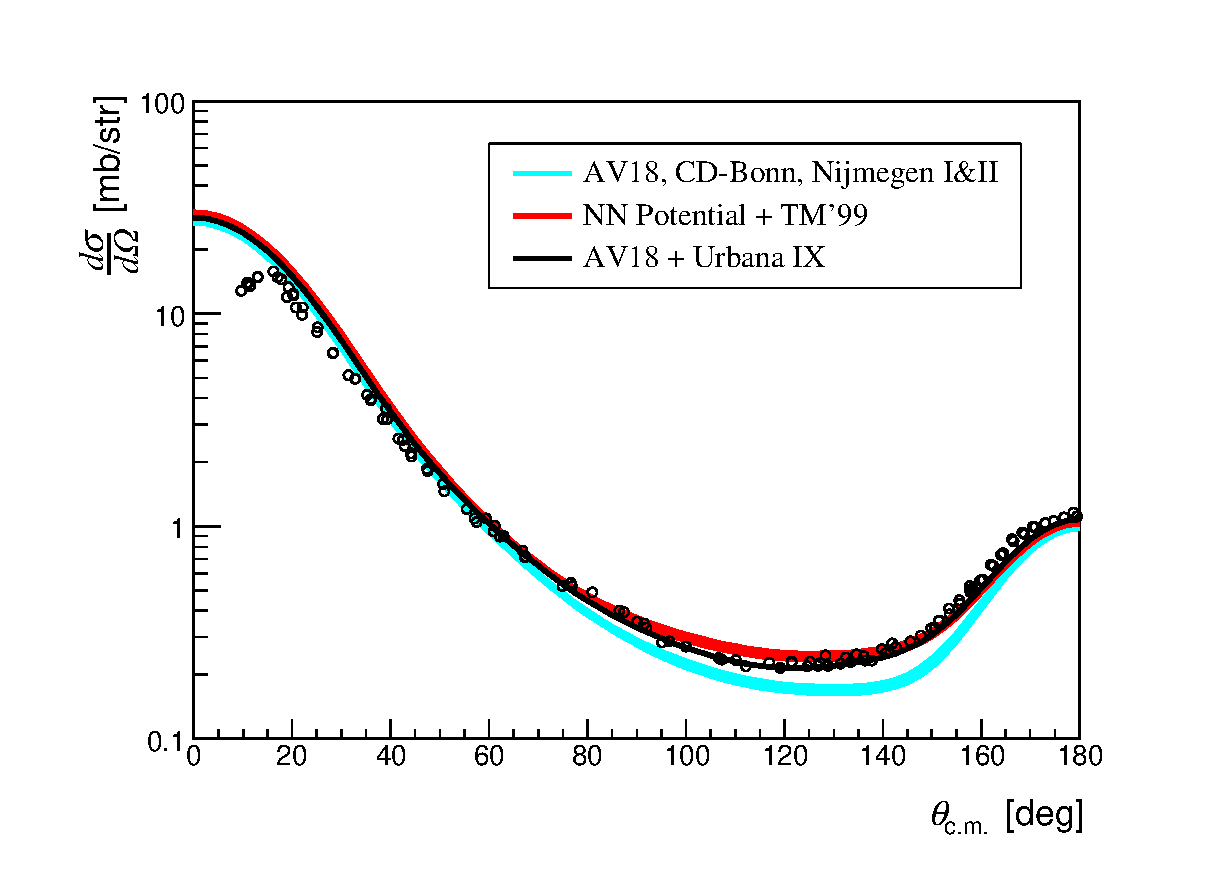
\includegraphics[clip,width=10cm]{./chap1/fig/dcs_dp_135MeV.eps}\\
%  \caption{核子当たり135 MeVでの重陽子--陽子弾性散乱の微分断面積\cite{Sek02}}
%  \label{dcs_dp135}
% \end{figure}

% %%%%%%%

% %% 1.2.3 %%
%   \subsection{四核子系散乱における三体核力}
% 近年では重陽子--陽子散乱のような三核子系だけでなく、四核子以上の核子系や、核物質の状態方程式においても三体核力の効果が重要視されている。例えば、質量数$A \sim 10$の軽い原子核の束縛エネルギーは、Green's Function Monte Carlo計算\cite{Pie01,PVW02}やNo-Core Shell Model計算\cite{NO03}などによって三体核力の効果を含んだ記述がなされており、その効果が無視できない大きさの寄与を与えるとされている。また中性子星の状態方程式においても三体核力による寄与が重要であることが示されており\cite{APR98}、中性子過剰な非対称核物質においては三体核力のアイソスピン依存性が重要となってくると示唆されている\cite{GCR12,Car15}。\\
%  我々のグループは、三体核力を含む核力から原子核という多体系を理論的に理解することを目指し、まず中間エネルギー領域における三体核力の性質を詳細に調べるため、実験プローブとして四核子である陽子--$^3$He散乱系を用いることにした。重陽子--陽子散乱では系のアイソスピンが$1/2$に限られているため、三体核力のアイソスピン依存性についてアプローチできない。しかし、陽子--$^3$Heのような四核子の散乱系では系のアイソスピンが$3/2$となるため、最終的には三体核力のアイソスピン依存性についてアプローチできると考えている。\\
%  陽子--$^3$Heの四核子散乱系については、Murdichらによって19.5 MeVから47.5 MeVの低エネルギー領域での弾性散乱における微分断面積が高精度で測定されている\cite{Mur84}。この測定による微分断面積はいずれも重陽子--陽子弾性散乱同様に$\theta_{\rm c.m.} \sim 120^\circ$で最小値を取っている。このことから中間エネルギー領域における陽子--$^3$He弾性散乱についても、微分断面積が最小値となる散乱角度において三体核力の効果を観測できると考えられる。\\
%  ここ数年では、三核子系だけでなく四核子の散乱系における観測量の厳密理論計算も可能になっている。およそ30 MeV以下での低エネルギー領域における陽子--$^3$He弾性散乱の観測量については、DeltuvaとFonseca\cite{DF13}やViviani\cite{Viv13}らによって理論計算が行われており、中間エネルギー領域において三体核力の効果が顕著に現れると予想されている。\\
%  中間エネルギー領域における陽子--$^3$Heの散乱系を系統的に調べていくために、まずこの散乱系の弾性散乱の完全測定を行うことを目標とした。完全測定とは、ある反応における散乱振幅のすべての要素が一意に決定できる測定である。このためには微分断面積だけでなく、偏極分解能などのスピン観測量の測定が必要不可欠である。偏極分解能とは反応に関わるいずれかの粒子がスピン偏極している時に観測される散乱の非対称を表す観測量である。偏極分解能の測定には、偏極ビームまたは偏極標的が必要となってくる。
  
% %%%%%%%

% %%%% 1.3 %%%%
%  \section{偏極${}^3$He標的}
% 前述のように我々のグループは、四核子系における三体核力の性質を詳細に調べていくために陽子--$^3$Heの散乱系の完全測定を目標とする。そのために、有効散乱角度における陽子--$^3$He弾性散乱での$^3$He偏極分解能測定を行う。我々は、この偏極分解能測定に必要不可欠である偏極$^3$He標的の開発を行ってきた。この節では、現在開発している偏極$^3$He標的に求められる条件および本研究以前の研究状況について述べる。

% %% 1.3.1 %%
%   \subsection{偏極$^3$He標的に要求される条件}
% 我々は測定によって得られた$^3$He偏極分解能の実験値と、理論計算によって得られた計算値とを比較することで、四核子系における三体核力の発現性について議論することを目的としている。そのためには高精度の実験データを得る必要がある。仮に$^3$He偏極分解能$A_y$をその統計誤差$dA_y$が0.02以下となるように測定することを要請した場合に、偏極標的に求められる条件について述べる。\\
%  陽子--偏極$^3$He弾性散乱における微分断面積は以下の式で与えられる。
% %
% \begin{equation}
%  \frac{d\sigma}{d\Omega} = \left( \frac{d\sigma}{d\Omega} \right)_0 ( 1+ {\bm p} \cdot {\bm A})
% \end{equation}
% %
% ここで$d\sigma/d\Omega$は$^3$He原子核が偏極している時の微分断面積で、添字の0は非偏極を表す。$\bm p$は$^3$He原子核の偏極度、$\bm A$はこの反応での$^3$He偏極分解能である。この式より、散乱角度$\theta$で散乱された陽子の検出数は、
% %
%  \begin{eqnarray}
%   L_{\rm up}=L_0[1+p_y A_y(\theta)] \\
%   L_{\rm down}=L_0[1-p_y A_y(\theta)] \\
%   R_{\rm up}=R_0[1-p_y A_y(\theta)] \\
%   R_{\rm down}=R_0[1+p_y A_y(\theta)]
%  \end{eqnarray}
%  %
% と表される。ここで、$L,R$ はビームの入射方向に対して左右に設置された検出器における散乱陽子の検出数である。左辺の添字は偏極方向の鉛直上向きおよび下向きを、右辺の0の添字は非偏極の場合を表す。またここでの座標系はマディソン規約\cite{Ohl72}に従い、ビームの入射軸を$z$軸、標的の偏極方向を散乱平面($xz$平面)に垂直な$y$軸に取っている(図\ref{madison}参照)。

% \begin{figure}[tbp]
%  \centering
%  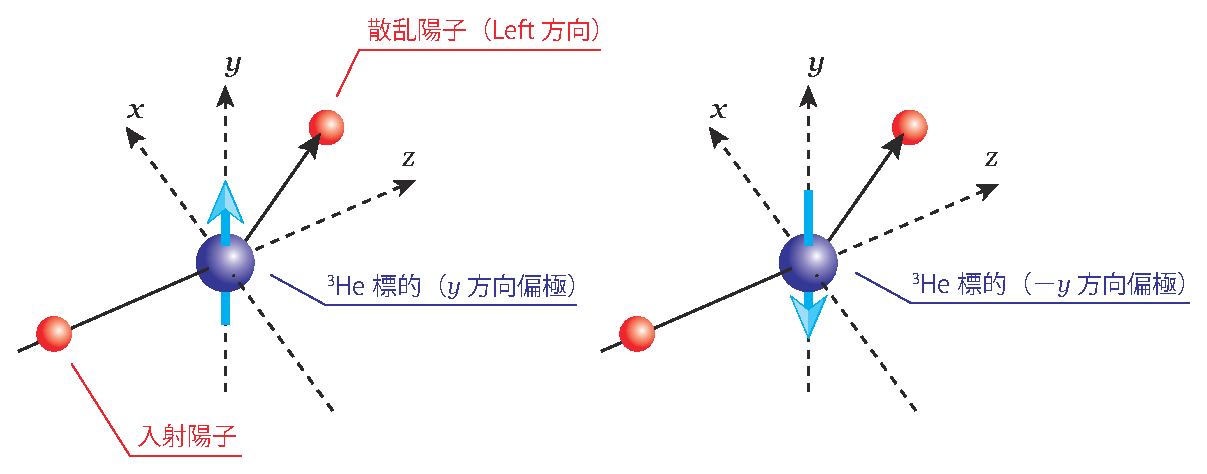
\includegraphics[clip,width=13cm]{./chap1/fig/madison.pdf}\\
%  \caption{マディソン規約から決定される陽子--偏極$^3$He散乱における座標系}
%  \label{madison}
% \end{figure}

% よって、これらの式から${}^3$Heの偏極分解能$A_y$は、次の式で求められる。
% %
%  \begin{equation}
%   A_y=\frac{1}{p_y} \frac{L_{\rm up}-L_{\rm down}}{L_{\rm up}+L_{\rm down}}=\frac{1}{p_y} \frac{R_{\rm down}-R_{\rm up}}{R_{\rm up}+R_{\rm down}}
%   \label{Ay_calc}
%  \end{equation}
%  %
% 偏極の向きを反転させれば、左右それぞれの検出器における反転前後の検出数の非対称度から偏極分解能を求めることができる。また偏極分解能の誤差$d A_y$は、次のように表される。
% %
%  \begin{eqnarray}
%   dA_y &=& \sqrt{\left( \frac{\partial A_y}{\partial Y_{\rm up}}\right)^2 (dY_{\rm up})^2+\left( \frac{\partial A_y}{\partial Y_{\rm down}}\right)^2 (dY_{\rm down})^2} \nonumber \\
%   (dA_y)^2 &=& \frac{1}{p_y^2} \frac{4}{(Y_{\rm up}+Y_{\rm down})^4}[Y_{\rm down}^2(dY_{\rm up})^2+Y_{\rm up}^2(dY_{\rm down})^2]
%   \label{Ay_err_1}
%  \end{eqnarray}
%  %
% ここで、左右の検出器において$dA_y$の表式は同じ形となるので、$Y=L,R$とした。$p_y A_y \ll 1$とすると、検出数の非対称度は小さくなるので、$Y \equiv Y_{\rm up} \sim Y_{\rm down}$となり、式(\ref{Ay_err_1})は
% %
%  \begin{equation}
%   (dA_y)^2 \sim \frac{1}{p_y^2} \frac{(dY)^2}{2Y^2}
%   \label{Ay_err_2}
%  \end{equation}
% %
% と近似できる。また検出器における粒子の検出数はPoisson分布に従うので、その統計誤差$dY_{\rm stat}$は$\sqrt{Y}$に等しくなる。よって式(\ref{Ay_err_2})は
% %
% \begin{equation}
%  (dA_y)^2 \sim \frac{1}{p_y^2} \frac{1}{2Y}
%  \label{Ay_err_3}
% \end{equation}
% %
% と表される。検出器における散乱粒子の検出数$Y$は次の式で表される。
% %
% \begin{eqnarray}
%  Y &=& N \cdot t \nonumber \\
%  &=& I \cdot \rho_{\rm T} \cdot \Delta \Omega \cdot \epsilon \cdot \frac{d\sigma}{d\Omega} \cdot t
%  \label{Yield}
% \end{eqnarray}
% %
% ここで$N$は単位時間あたりの散乱粒子の検出数、$t$は測定時間である。また$I$は入射粒子のフラックス、$\rho_{\rm T}$は標的粒子の単位面積あたりの数密度、$\Delta \Omega$は検出器の立体角、$\epsilon$は散乱粒子の検出効率で、$d\sigma/d\Omega$は微分断面積である。式(\ref{Yield})を式(\ref{Ay_err_3})に代入すると、$^3$He偏極分解能$A_y$の統計誤差は
% %
% \begin{equation}
%  (dA_y)^2 \sim \frac{1}{2p_y^2 \cdot \rho_{\rm T}} \frac{1}{I \cdot \Delta \Omega \cdot \epsilon \cdot \cfrac{d\sigma}{d\Omega} \cdot t}
%  \label{Ay_err_4}
% \end{equation}
% %
% となる。標的に関するパラメーターを見ると、$A_y$の統計誤差の2乗は標的粒子の単位面積あたりの数密度$\rho_{\rm T}$と標的の偏極度$p_y$の2乗の積に反比例する。よって、統計誤差を小さくするためには高密度かつ高偏極度の標的が必要となる。\\
%  次に、式(\ref{Ay_err_4})を用いて$^3$He偏極分解能の統計誤差$dA_y$が0.02以下となる時に要請される標的の条件を求める。標的以外(実験条件および測定系)に関するパラメーターについては、表\ref{para_Ay}のような値を仮定した。表\ref{para_Ay}の値を式(\ref{Ay_err_4})に代入すると、

% \begin{table}[htbp]
%  \caption{実験条件および測定系に関するパラメーターの仮定値}
%  \centering
%   \begin{tabular}{|c|c|} \hline
%   名称 & 仮定した値 \\ \hline \hline
%   測定時間 $t$ & 5時間 \\
%   ビーム強度 $I \cdot e$ & 5 nA \\
%   検出器の立体角 $\Delta \Omega$ & 0.5 msr \\
%   検出効率 $\epsilon$ & 100% \\
%   微分断面積 $d\sigma/d\Omega$ & 0.5 mb/sr \\ \hline
%   \end{tabular}
%  \label{para_Ay}
% \end{table}

% %
% \begin{eqnarray}
%  (dA_y)^2 &\sim& \frac{1}{2p_y^2 \cdot \rho_{\rm T}} \frac{1}{\cfrac{5 \times 10^{-9}}{1.6 \times 10^{-19}} \cdot 0.5 \times 10^{-3} \cdot 1 \cdot 0.5 \times 10^{-27} \cdot 5 \times 60^2} \nonumber \\
%   &\simeq& \frac{3.56 \times 10^{15}}{p_y^2 \cdot \rho_{\rm T}}
%   \label{Ay_err_5}
% \end{eqnarray}
% %
% となる。ここで、$^3$Heの原子量は3.015 g/molなので、標的の密度を$\rho~{\rm g/cm^3}$、長さを$l~{\rm cm}$とすると、
% %
% \begin{eqnarray}
%  (dA_y)^2 &\sim& \frac{3.56 \times 10^{15}}{p_y^2 \cdot \rho_{\rm T}} \nonumber \\
%  &=& \frac{3.56 \times 10^{15}}{p_y^2 \cdot \rho \cdot l \cdot \cfrac{6.022 \times 10^{23}}{3.015}} \nonumber \\
%  &\simeq& \frac{1.78 \times 10^{-8}}{p_y^2 \cdot \rho \cdot l}
%  \label{Ay_err_6}
% \end{eqnarray}
% %
% と計算できる。式(\ref{Ay_err_6})において、$dA_y<0.02$を要請すると、結局標的に求められる条件は次の式で表される。
% %
% \begin{equation}
%  p_y^2 \cdot \rho \cdot l > \frac{1.78 \times 10^{-8}}{(0.02)^2} = 4.45 \times 10^{-5}
%  \label{tar_cond}
% \end{equation}
% %
% $0$℃、$1$気圧における$^3$Heの密度は$1.35 \times 10^{-4}~{\rm g/cm^3}$であるから、$^3$Heガスの圧力を$3$気圧、標的の長さを$2~{\rm cm}$程度とすると、25%程度の偏極度が得られれば要請した統計誤差を満たす。\\
%  また式(\ref{Ay_calc})より、偏極分解能の値を求めるためには標的の偏極度が既知でなければならない。散乱実験が数十時間に渡って行われるものだとすれば、実験中に標的の偏極度を測定できるシステムが必要である。

% %%%%%%%

% %% 1.3.2 %%
%   \subsection{これまでの研究状況}
% 我々のグループは$^3$Heの偏極分解能の高精度測定のために、以上の条件を満たす偏極$^3$He標的の開発を行ってきた。これまでの開発で、$^3$Heガスを封入したガラスセルを作成し、スピン交換光ポンピング法による$^3$Heの偏極生成に成功している\cite{wada}。$^3$Heの偏極は、高速断熱通過-核磁気共鳴(AFP-NMR)法による測定を行うことで確認した。しかしAFP-NMR法による測定では$^3$He偏極度に対応した大きさの信号しか得られないので、偏極度の絶対値を求めることができない。そこでこの偏極$^3$He標的を用いて、$35~{\rm MeV}$の陽子ビームによる陽子--$^3$He弾性散乱実験を行った。$35~{\rm MeV}$での陽子--$^3$He弾性散乱における$^3$He偏極分解能はMcCamisらによって制度良く測定されており\cite{McC85}、この値から偏極度の絶対値を求めることができる。McCamisらによる$^3$He偏極分解能の測定結果を図\ref{Ay_35MeV}に示す。実験の結果、標的の偏極による散乱の非対称は観測されず、$^3$Heの偏極度が1%以下の非常に低い値であることが分かった。\\

% \begin{figure}[tbp]
%  \centering
%  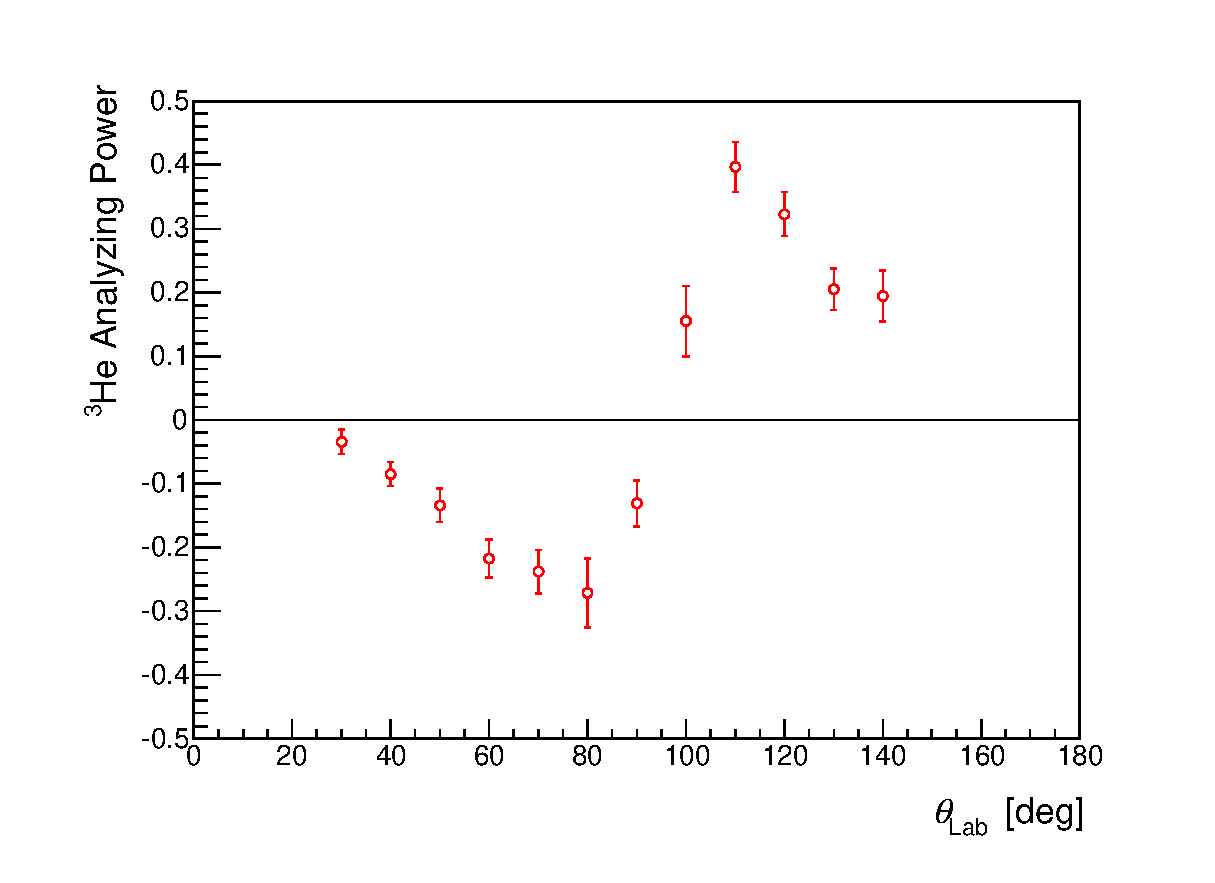
\includegraphics[clip,width=10cm]{./chap1/fig/Ay_p+3He_35MeV.eps}\\
%  \caption{$35~{\rm MeV}$の陽子--$^3$He弾性散乱における$^3$He偏極分解能\cite{McC85}}
%  \label{Ay_35MeV}
% \end{figure}

% これを受け、我々は$^3$He偏極度の向上のために偏極度シミュレーションによるガラスセルの最適化を行った\cite{shiokawa}。$^3$Heガスを封入するガラスセルの形状の最適化をすることで、効率よく光ポンピングを行い、結果的に$^3$He偏極度を向上させることを目的とした。これによって最適化されたガラスセルを新たに作成し、再び$35~{\rm MeV}$の陽子ビームによる陽子--$^3$He弾性散乱実験を行った。その結果、標的の偏極による散乱の非対称が観測された。しかし、同様に既知の$35~{\rm MeV}$での$^3$He偏極分解能から偏極度を求めた結果、およそ5%という値が得られ、要請された条件を満たしていないことが明らかとなった。

% %%%%%%%
% %%%%%%%%%%

% %%%% 1.4 %%%%
%  \section{本研究の目的}
% 以上のように、我々のグループが開発した偏極$^3$He標的は要請された条件を満たしておらず、偏極度の向上が必要である。また現在$^3$Heの偏極度を測定する方法として採用しているAFP-NMR法のみでは、偏極度の相対値しか求められない。現状では既知の$^3$He偏極分解能が得られている$35~{\rm MeV}$での陽子--$^3$He弾性散乱実験を行い、実験で得られた散乱の非対称から、標的の偏極度の絶対値を求める方法を取っている。しかしこの方法では偏極度の絶対値を得るために散乱実験を行わなければならず、また散乱の非対称は小さいので高精度で偏極度を得るのは困難である。最終的に中間エネルギー領域における$^3$He偏極分解能を高精度で得るためには、同様に高精度で$^3$He偏極度の絶対値を求める必要がある。偏極度の向上を目指すにあたっても容易に偏極度を測定できるシステムの構築が必要不可欠である。よって、本研究では新たな$^3$He偏極度測定システムを導入し、得られた偏極度からAFP-NMRの較正を行うことを目的とする。新たに導入する測定システムとして、Rbの電子スピン共鳴(ESR)を利用した$^3$He偏極度測定を採用した。また$^3$He偏極度の測定精度としては$10$%以下を目標とした。\\
%  以降の本稿の構成について簡潔に述べる。第2章では$^3$He原子核のスピン交換光ポンピング法による偏極生成の原理、またAFP-NMR法や本研究で導入するRbのESRを利用した$^3$He偏極度測定の原理について述べる。第3章では我々のグループにおける偏極$^3$He標的装置および標的製作装置について述べる。第4章では製作した標的を用いた偏極生成および新たに導入した$^3$He偏極度測定について述べる。第5章では東北大学サイクロトロンRIセンター(CYRIC)において行った$70~{\rm MeV}$の陽子ビームを用いた陽子--$^3$He弾性散乱実験について述べる。第6章では今回導入した$^3$He偏極度測定システムおよび偏極標的についての考察を述べ、第7章で本研究のまとめを述べる。

% %%%%%%%%%%
